\subsection{Astrobiology System}
\label{sec:Astrobiology System}

\subsubsection{Design and Operation}
The collection assembly will be designed as a multi-compartment structure, with various collection and control containers, two pumps, two pump heaters, and two solenoids.  The control containers will be connected to a solenoid that will remain closed until post-sanitation procedures are performed. The sample collection containers will be connected to a vacuum pump located outside of the clean box structure.  One of the chambers will be a non-liquid collection container. Heaters will be attached to the pumps to aid during a cold start. Once float altitude is reached, the solenoids connected to the sample collection containers will be opened and the pumps will be powered on; allowing air to flow to the collection containers. The containers will hold a range of amounts and concentrations, \SIrange{30}{60}{\milli\liter} of \SIrange{15}{30}{\%} sterile glycerol solutions. A 316 Stainless Steel \SI{1/4}{\inch} NPT Vent to Atmosphere Vitron Seal Valve will be embedded in each of the compartments, to accommodate for the pressure changes that occurs with the variations in altitude over the course of a flight~\cite{valve}, as well as operate as the sample exhaust.  The left side of Figure~\ref{fig:pump} displays the collection assembly with the openings for the sample and exhaust tubing, while the right side of Figure~\ref{fig:pump} shows the 3D rendering of the sampling pump.  

\begin{figure}[!h] 
\begin{center}
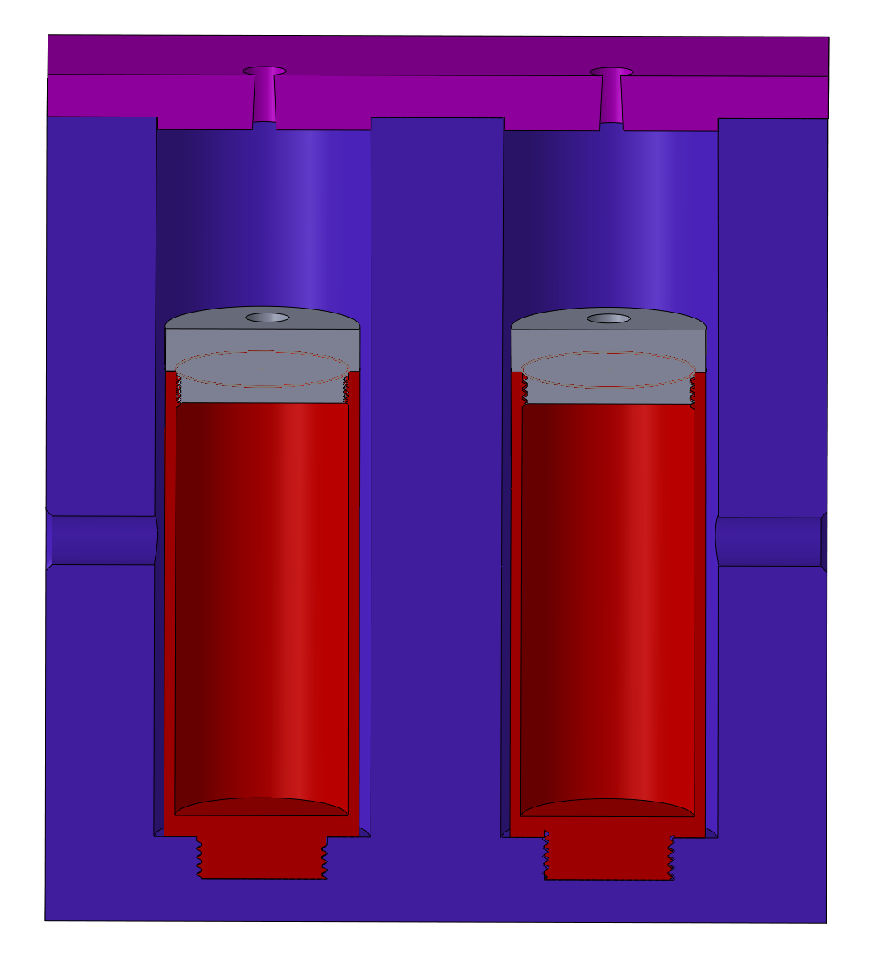
\includegraphics[scale=.4]{./Figures/CB.PDF}
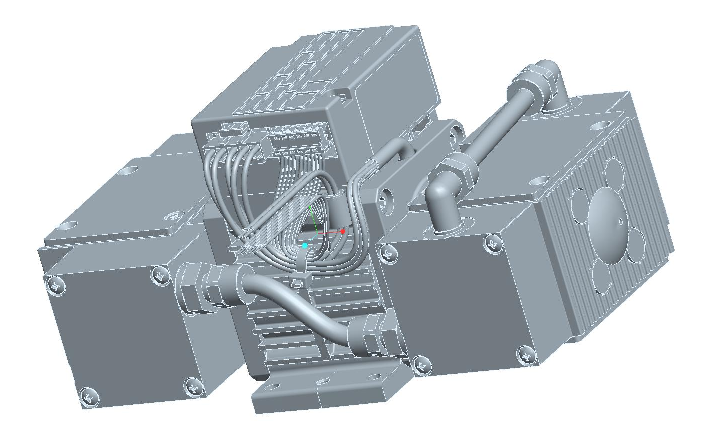
\includegraphics[scale=.8]{./Figures/Pump.pdf}
\caption{{\bf Left:} Cross-section view of the clean box with experimental and control containers. {\bf Right:} KNF N84-4 commercial gas-sampling diaphragm vacuum pump. \cmt{Andrew R}{This figure is also not showing up, not sure why...}}
\label{fig:pump}
\end{center}
\end{figure} 
%\subsection{Astrobiology Methods}
%\label{sec:Astrobiology Methods}
\subsubsection{Pre-Flight Preparation}

The clean box, collection containers and tubing will be autoclaved. All tools used in the assembly of the clean box will either be autoclaved or soaked in a \SI{70}{\percent} ethanol solution inside of a clean room. Each person who enters the clean room will be garbed in a lab coat, goggles, hair net and latex gloves after thoroughly washing their hands in a \SI{70}{\percent} ethanol solution. 

We will varry the glycerol concentration and increase the amount of medium within the assembly.  The \SI{15}{\percent}, \SI{25}{\percent}, and \SI{30}{\percent} glycerol solutions will be poured into each container, the lid will then be sealed with silicone gasket maker along with the tubing inserted and gasket sealed into the container lids. Each lid will have two holes, one that leads to the inside of the clean box to allow for pressure to be released from inside the container and outgassed through the valve that will be embedded in the box, while the other hole will be passed through the clean box lid to allow the tubing to connect to the pump - solenoid system only in the case of the control tubing. The lid to the clean box willl be sealed with silicone gasket maker, the box will be mounted onto the payload and the tube from the control container will be clamped to the dedicated control solenoid, while the sample collecting tube will be passed through the other solenoid and connect to the pump. A final piece of tubing will be connected from the intake valve on the pumps to the outside of the payload, after a \SI{70}{\percent} ethanol solution is ran through the pump several times. The end of the tubing will connect to a mechanism that will isolate the inner tubing until float conditions are reached. The payload will then be closed and remain  in the clean room until it is ready for transport flight.

\subsubsection{Post Flight Procedures}

Once the payload is retrieved, the intact clean box needs to be removed and placed inside of a cooler with ice to be then transported to The University of Houston and placed in cold storage at \SI{4}{\celsius}. All equipment used in the filtration process will be either autoclaved or taken from previously unopened sanitized packaging. The autoclaved, pre-sanitized items and the clean box will then be washed in a \SI{70}{\percent} ethanol solution before they are placed inside a SterilGARD e3 Class II Biological Safety Cabinet (the Cabinet). The cabinet has a laminar flow air barrier and UV lights built into the ceiling for decontaminating the workspace prior to use. A portion of both the control and sample collection solutions will be vacuum filtered through a Fluropore membrane filter (\SI{13}{\milli\meter}; \num{0.22} micron) to collect specimens on the filter surface.  The filters will then packaged for in-house 16S ribosomal RNA sequencing.  In addition, the remaining portion of the glycerol solutions will be used on various culturing media in an attempt to culture any microbes that are collected.
